\section{Одномерные дискретные динамические системы}

Пусть задана функция $f$, $f(t): \: X \to Y$, $X, Y \in \mathbb{R}$. Имеем систему

\begin{equation}
\begin{cases}
\label{ch1.sys}
N_{t+1} = f(N_t)&\\
N(0) = N_0&
\end{cases}
\end{equation}
где $t = 0, 1, \ldots$ Это и есть одномерная дискретная динамическая система.

\textbf{Примеры:}
\begin{itemize}

\item Логистический закон.

\begin{equation*}
N_{t + 1} = 2 N_t \left(1 - \frac{N_t}{k} \right)
\end{equation*}
$k$~---~ресурс.

\item Отображение Рикера.

\begin{equation*}
N_{t+1} = N_t e^{r \left(1 - \frac{N_t}{k}\right)}
\end{equation*}

\end{itemize}

\begin{figure}[h]
\begin{center}
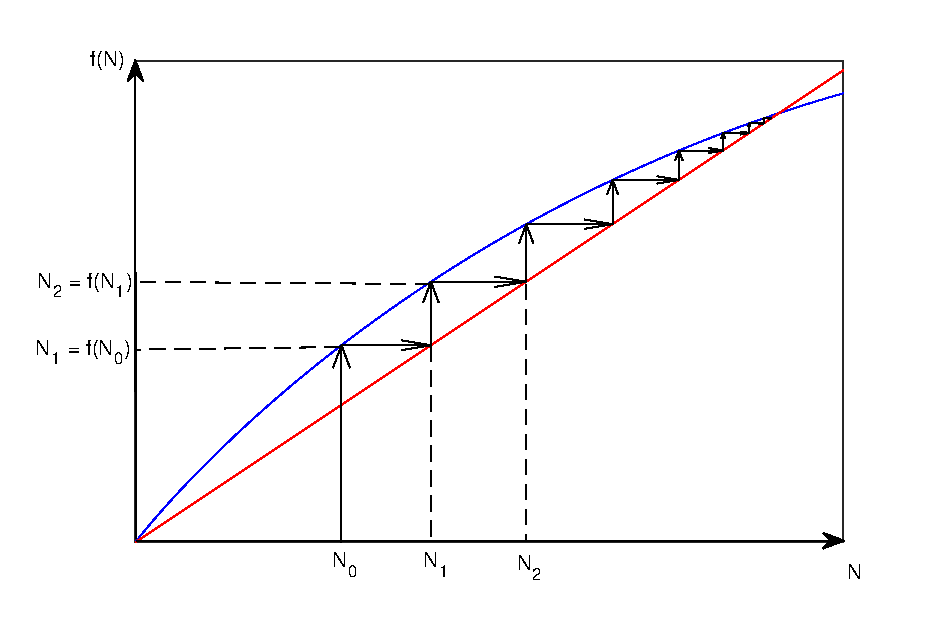
\includegraphics[width=0.8\linewidth]{ch1/ch1_fig1.eps}
\caption{Графическая процедура построения решения}
\label{ch1.fig1}
\end{center}
\end{figure}


\begin{definition}
Точка $N^*$ системы (\ref{ch1.sys}) называется \textit{неподвижной}, если $N^* = f(N^*)$.
\end{definition}


\begin{definition}
Неподвижная точка $N^*$ называется \textit{устойчивой (по Ляпунову)}, если $\forall \varepsilon > 0$ существует $\delta(\varepsilon): \: \forall N_0 \in \cup^\delta_{N^*}$, верно $|N_t - N^*| < \varepsilon, \, \forall t$.
\end{definition}

\begin{definition}
Неподвижная точка $N^*$ называется \textit{асимптотически устойчивой}, если она устойчива по Ляпунову и $\lim\limits_{t \to + \infty} N_t = N^*$.
\end{definition}

\begin{theorem}[достаточное условие устойчивости]
\label{ch1.th1}
Пусть $N^*$~---~неподвижная точка $f$, т.е. $f(N^*) = N^*$. Тогда
\begin{itemize}

\item если $|f'(N^*)|<1$, то $N^*$~---~асимптотически устойчива;
\item если $|f'(N^*)|>1$, то $N^*$~---~неустойчива;
\item если $|f'(N^*)|=1$, то ничего сказать нельзя.

\end{itemize}	
\end{theorem}
\begin{proof}

Дано
\begin{equation}
\label{ch1.th1.cond1}
N_{t+1} = f(N_t), \, t = 0, 1, 2, \ldots
\end{equation}
Также дано, что $N^*$~---~неподвижная, т.е.
\begin{equation}
\label{ch1.th1.cond2}
N^* = f(N^*)
\end{equation}

Введём следующие обозначения: $\Delta N_{t+1} = N_{t+1} - N^*$, $\Delta N_{t} = N_{t} - N^*$. Тогда 

\begin{equation*}
\begin{aligned}
&N_{t+1} = N^* + \Delta N_{t+1}, \\
&N_{t} = N^* + \Delta N_t.
\end{aligned}
\end{equation*}

Перепишем (\ref{ch1.th1.cond1}) при помощи наших новых обозначений
\begin{equation*}
N^* + \Delta N_{t+1} = f(N^* + \Delta N_t) = f(N^*) + f'(N^*) \Delta N_t + \overline{\overline{o}}(\Delta N_t),
\end{equation*}
И с учётом (\ref{ch1.th1.cond2}) 
\begin{equation*}
\Delta N_{t+1} = f(N^* + \Delta N_t) = f'(N^*) \Delta N_t + \overline{\overline{o}}(\Delta N_t).
\end{equation*}

Разделим это уровнение на $\Delta N_t$ и получим
\begin{equation*}
\frac{\Delta N_{t+1}}{\Delta N_t} = f'(N^*) + \frac{\overline{\overline{o}}(\Delta N_t)}{\Delta N_t}.
\end{equation*}

В силу сходимости $\frac{\overline{\overline{o}}(\Delta N_t)}{\Delta N_t}$ к $0$ при $\Delta N_t \to 0$, можем сказать, что $\frac{\Delta N_{t+1}}{\Delta N_t} = f'(N^*)$. Это нам даёт, что при $\left|\frac{\Delta N_{t+1}}{\Delta N_t}\right| > 1$ мы удаляемся от $N^*$, а при $\left|\frac{\Delta N_{t+1}}{\Delta N_t}\right| < 1$~---~приближаемся. Откуда следует, что теорема доказана.
\end{proof}

\subsection*{Модель взаимодействия загрязнения с окружающей средой}
$u$~---~загрязнение, $f_1 = f(u)$~---~что выбрасывается.
\begin{equation*}
\begin{aligned}
&f_2(u) = f(u + f_1(u)),\\
&\qquad \ldots\\
&f_n(u) = f(u + f_{n-1}(u)).
\end{aligned}
\end{equation*}

Оценим сдвиг. Предположим, что $f(u) \leq au + b$, тогда 
\begin{equation*}
\begin{aligned}
&f_1(u) \leq ax + b,\\
&f_2(u) \leq a(u + f_1(u)) + b = a(u + au + b) + b = u(a + a^2) + b(a + 1),\\
&\qquad \ldots\\
&f_n(u) \leq u(a + a^2 + \ldots + a^n) + b(a + a^2 + \ldots + a^n + 1).
\end{aligned}
\end{equation*}
Если $a < 1$, то $f_n(u) \to \frac{au}{1 - a} + \frac{b}{1 - a} = \frac{au + b}{1 - a}$.

\begin{figure}[H]
\begin{center}
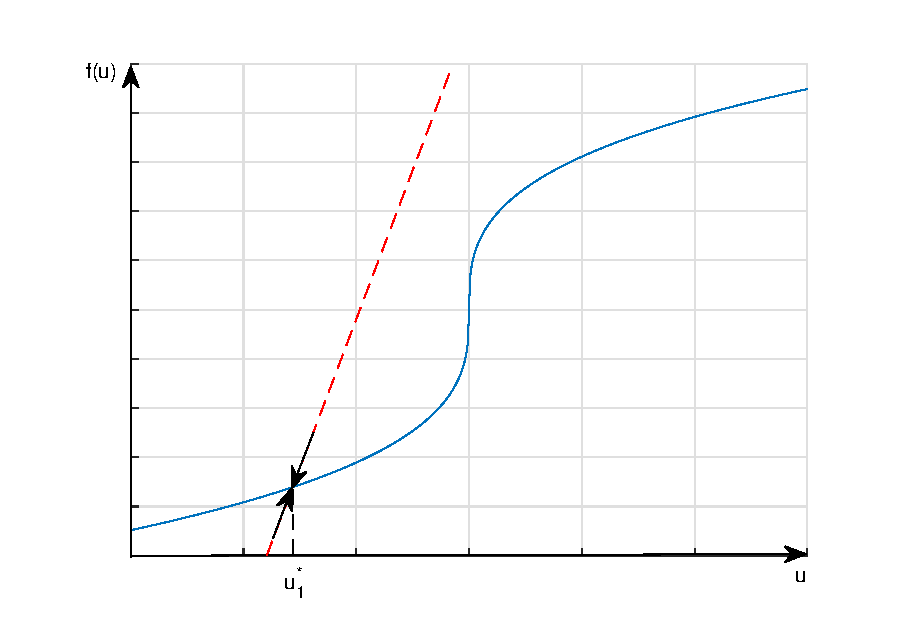
\includegraphics[width=0.5\linewidth]{ch1/ch1_fig2.eps}
\caption{$u_1^*$~---~устойчивая точка (точка природного очищения)}
\label{ch1.fig2}
\end{center}
\end{figure}

\begin{figure}[H]
\begin{center}
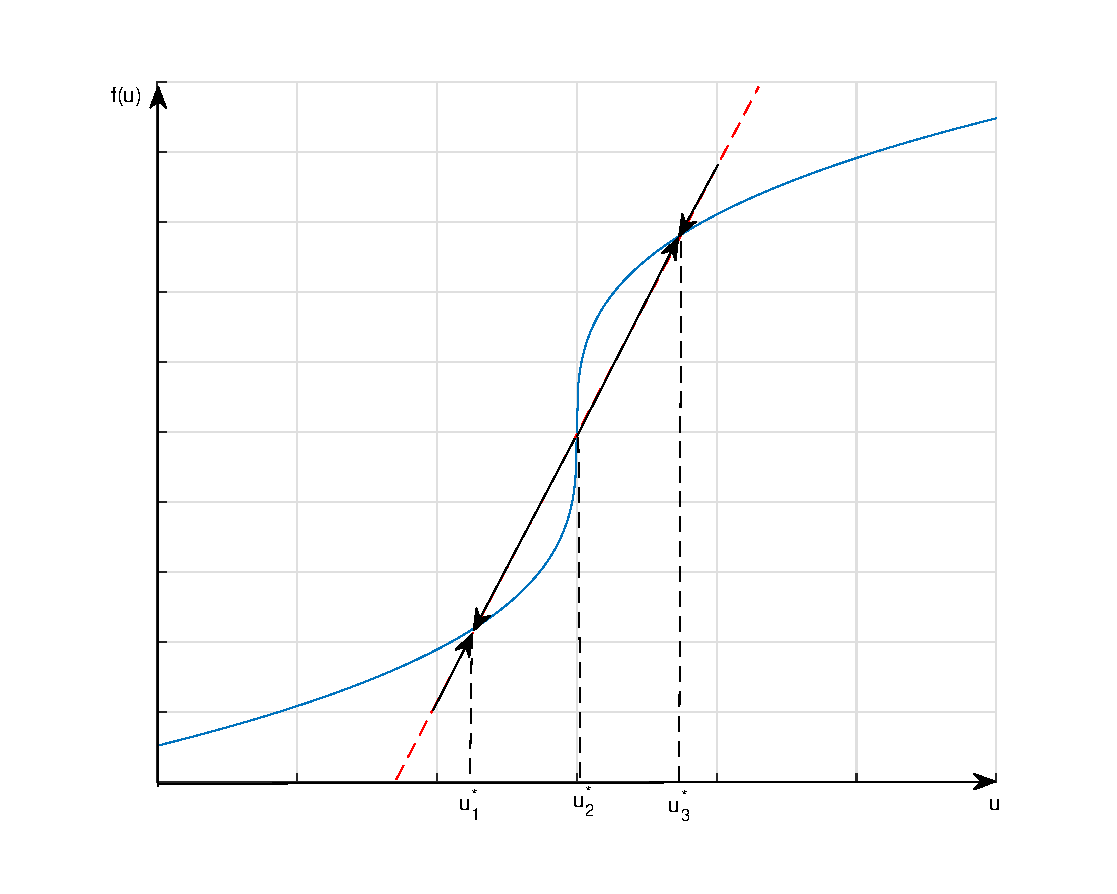
\includegraphics[width=0.5\linewidth]{ch1/ch1_fig3.eps}
\caption{$u_1^*$, $u_3^*$~---~устойчивые точки, $u_2^*$~---~неустойчивая.}
\label{ch1.fig3}
\end{center}
\end{figure}

\pagebreak

\begin{figure}[t]
\begin{center}
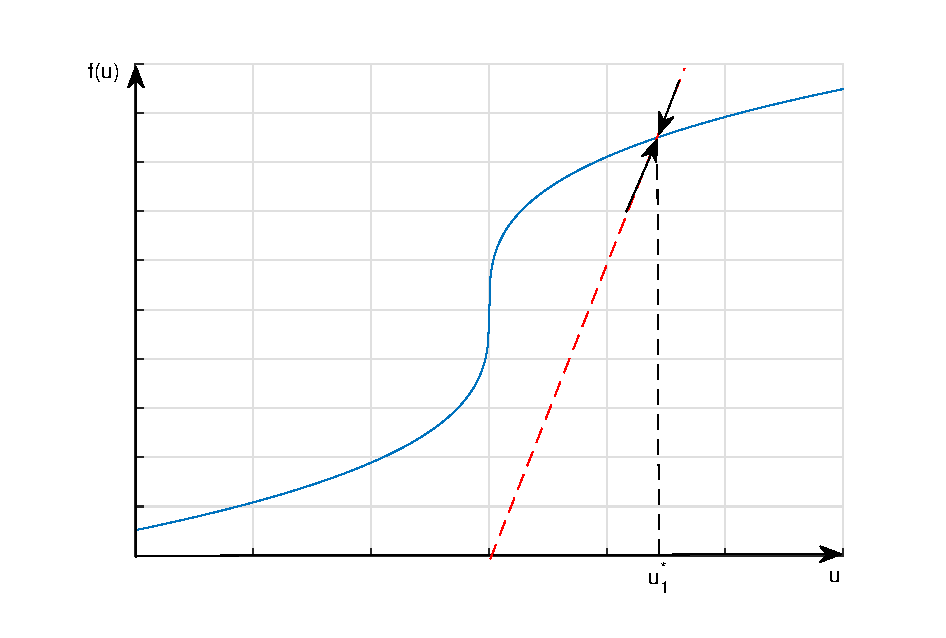
\includegraphics[width=0.5\linewidth]{ch1/ch1_fig4.eps}
\caption{$u_1^*$~---~точка устойчивого загрязнения}
\label{ch1.fig4}
\end{center}
\end{figure}

\subsection*{Дискретное логистическое отображение}
\begin{multicols}{2}
\begin{equation*}
\begin{aligned}
&u_{t+1} = ru_t (1 - u_t), \, r>0, \, 0 \geq u_t geq 1\\
&u^* = r u^* (1 - u^*)\\
&u_1^* = 0\\
&u_2^* = \frac{r - 1}{r} (\text{существует при}\, r>1
\end{aligned}
\end{equation*}

\begin{equation*}
\begin{aligned}
&f(u) = ru(1 - u)\\
&f'(u) = r - 2ru\\
&f'(u_1^*) = f'(0) = r < 1\\
&f'(u_2^*) = r - 2r \frac{r - 1}{r} = -r + 2, \, 1<r<3
\end{aligned}
\end{equation*}
\end{multicols}

\begin{figure}[h]
\begin{center}
\begin{minipage}[h]{0.49\linewidth}
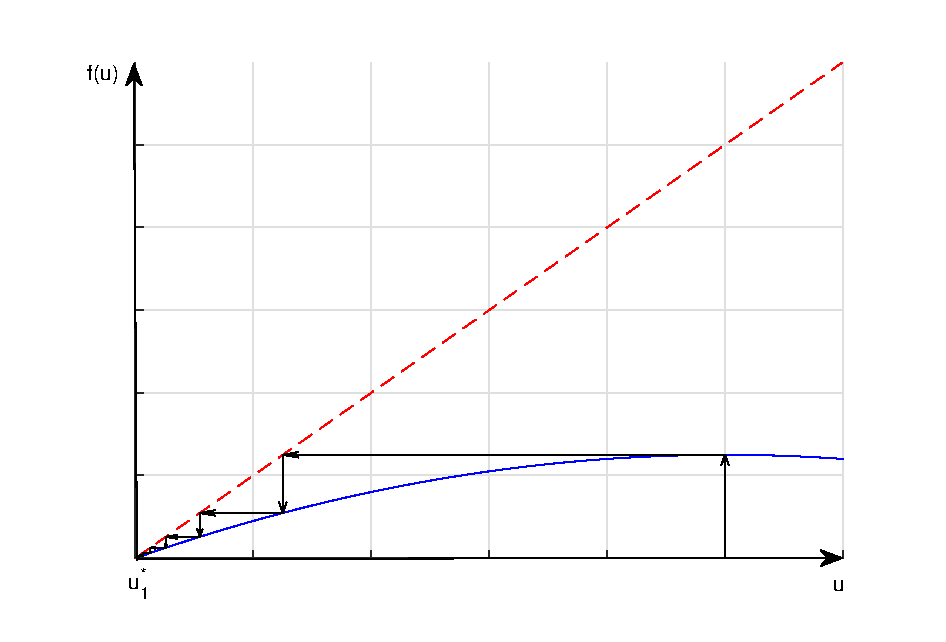
\includegraphics[width=1\linewidth]{ch1/ch1_fig5.eps}
\caption{Поведение системы при $r < 1$,\\ $u_1^*$~---~неустойчивая точка}
\label{ch1.fig5}
\end{minipage}
\hfill
\begin{minipage}[h]{0.49\linewidth}
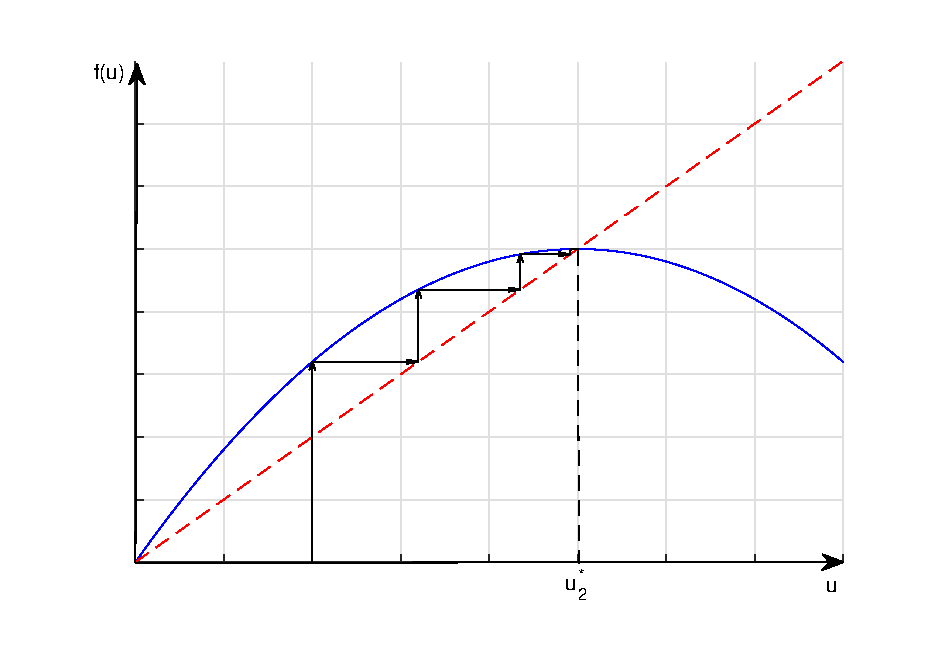
\includegraphics[width=1\linewidth]{ch1/ch1_fig6.eps}
\caption{Поведение системы при $1 < r < 3$, $u_2^*$~---~устойчивая точка}
\label{ch1.fig6}
\end{minipage}
\end{center}
\end{figure}

\begin{definition}
Набор $(V_1, V_2, \ldots, V_k)$ образуют цикл длины $k$, если 
\begin{equation*}
\begin{aligned}
&V_2 = f(V_1)\\
&V_3 = f(V_2)\\
&\quad \ldots\\
&V_k = f(V_{k-1})\\
&V_1 = f(V_{k})
\end{aligned}
\end{equation*}
то есть
\begin{equation*}
V_1 = f(f(\ldots f(f(V_1))\ldots)) = f^k(V_1)
\end{equation*}
\end{definition}

В нашем случае имеем:
\begin{equation*}
\begin{aligned}
&u_2 =ru_1(1 - u_1)\\
&u_1 =ru_2(1 - u_2)\\
&u_1 = rru_1(1 - u_1)(1 - r u_1 (1 - u_1))
\end{aligned}
\end{equation*}

Рассмотрим график:\\
\begin{figure}[H]
\begin{center}
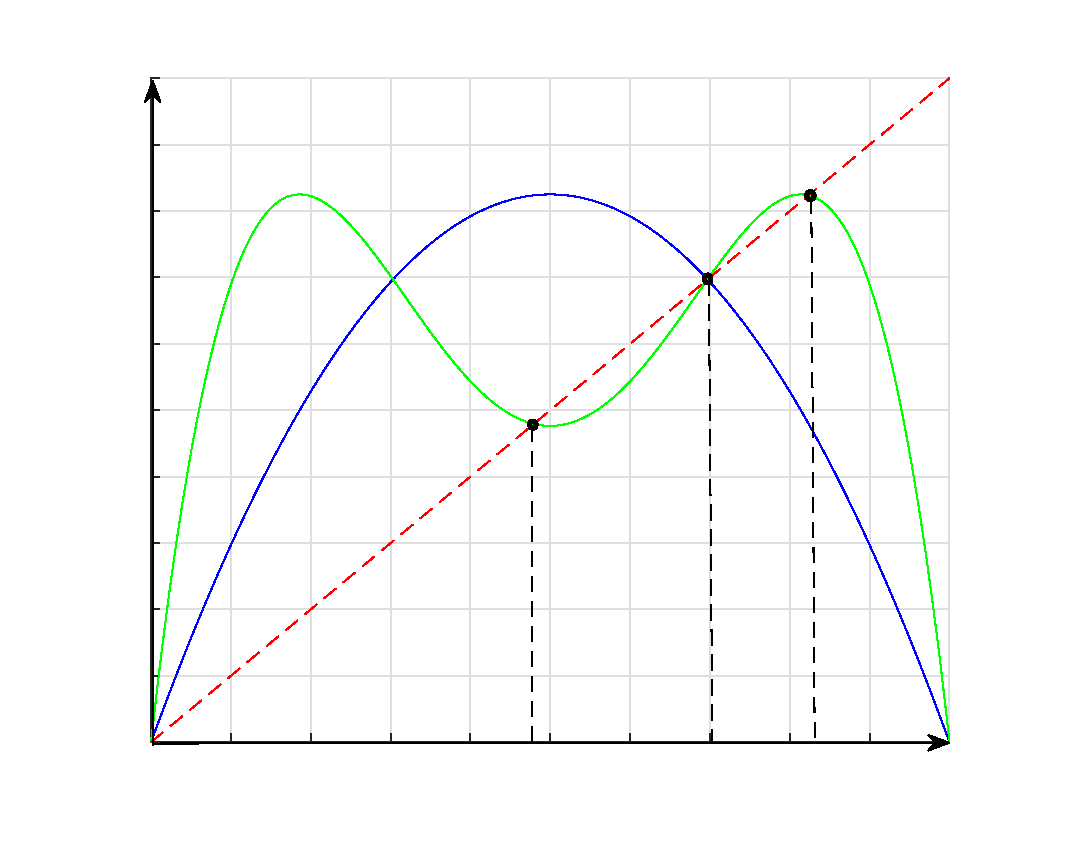
\includegraphics[width=0.5\linewidth]{ch1/ch1_fig7.eps}
\label{ch1.fig7}
\end{center}
\end{figure}
На графике изображены $f(u)$, $f^2(u)$ и прямая $u$. Явно видно наличие цикла длины 2. То есть $f(u^*) = u^*$, $f^2(u^*) = f(f(u^*)) = f(u^*) = u^*$.

\begin{assertion}
Любая точка цикла является неподвижной точкой отображения $f^k = f(f(\ldots ))$~---~суперпозиция.
\end{assertion}

\begin{definition}
Цикл называется \textit{устойчивым по Ляпунову}, если неподвижные точки $u_i$, $i = \overline{1,k}$ являются устойчивыми для $f^k$.
\end{definition}
\begin{assertion}[достаточное условие устойчивости]
 $\left| \frac{d}{du} f^k (u)|_{u = u_i}\right| < 1$
\end{assertion}
\begin{proof}
$\frac{d}{du} f^k (u_1) = f'(u_1) f'(u_2) \ldots f'(u_k) < 1$. Далее из теоремы \ref{ch1.th1} следует доказательство этого утверждения.
\end{proof}

В случае логистического отображения $f(u) = ru(1 - u)$, $f^2 (u) = r(ru(1-u))(1-ru(1-u))$. Здесь есть цикл длины 2.
\begin{equation*}
\begin{aligned}
&ru^3 + 2ru+(r+1)u + \frac{1}{r^2} + 1 = 0\\
&u_2 = \frac{r - 1}{r}
\end{aligned}
\end{equation*}
Можно поделить на $u - \frac{r - 1}{r}$. Другие корни
\begin{equation*}
u_{3,4} = \frac{r+1 \pm \sqrt{r^2 - 2r - 3}}{2r}
\end{equation*}
При $3 < r < 1 + \sqrt{6}$ есть цикл длины 2, при $r > 1 + \sqrt{6}$ есть циклы длинны 4, 8, 3, 7,\ldots

\begin{figure}[H]
\begin{center}
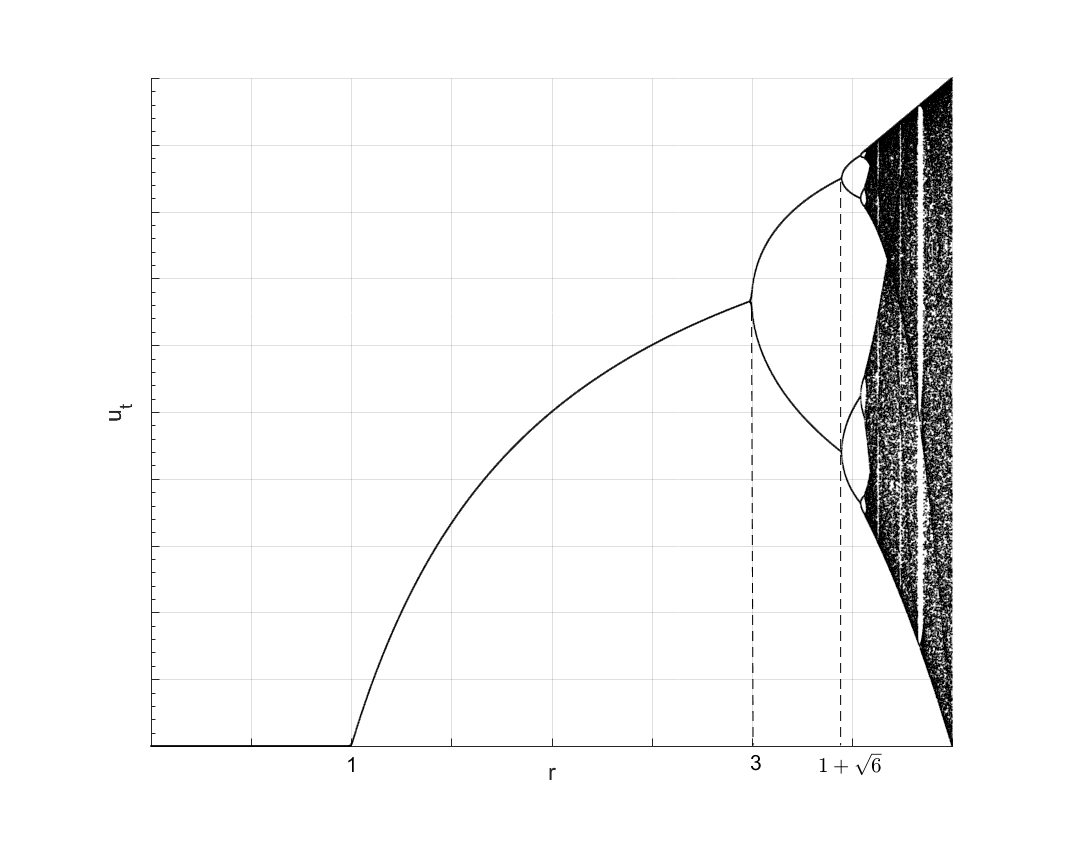
\includegraphics[width=0.5\linewidth]{ch1/ch1_fig8.eps}
\caption{Бифуркационная диаграмма}
\label{ch1.fig8}
\end{center}
\end{figure}

\section{Теорема Шарковского}

\begin{definition}
Будем говорить, что все натуральные числа \textit{упорядочены по Шарковскому}, если
\begin{equation*}
\begin{aligned}
& 3 \succ 5 \succ 7 \succ \ldots \succ \hfill \text{все нечётные числа, кроме }1 &\\
& \succ 2 \cdot 3 \succ 2 \cdot 5 \succ 2 \cdot 7 \succ \ldots \succ \text{все нечётные числа, умноженные на }2\text{, кроме }1 &\\
& \succ 2^2 \cdot 3 \succ 2^2 \cdot 5 \succ 2^2 \cdot 7 \succ \ldots \succ \text{все нечётные числа, умноженные на }2^2\text{, кроме }1 &\\
& \succ 2^3 \cdot 3 \succ 2^3 \cdot 5 \succ 2^3 \cdot 7 \succ \ldots \succ \text{все нечётные числа, умноженные на }2^3\text{, кроме }1 &\\
& \succ \ldots \succ &\\
& \succ 2^3 \succ 2^2 \succ 2 \succ 1. &\\
\end{aligned}
\end{equation*}
\end{definition}

\begin{theorem}[теорема Шарковского]
Пусть $f: \: \mathbb{R} \rightarrow \mathbb{R}$~---~непрерывное отображение, и пусть $f$ имеет цикл длины $k$. Тогда $f$ имеет цикл длины $m$ для всех таких $m$, что $k \succ m$ в указанном выше порядке.

Из теоремы непосредственно следует, что если отображение имеет цикл длины 3, то существуют циклы любой длины. Если отображение не имеет цикла длиной 2, то циклов нет вообще.
\end{theorem}

\section{Показатели и числа Ляпунова}

Рассмотрим два процесса:
\begin{multicols}{2}
\begin{equation*}
\begin{cases}
u_{t+1} = f(u_t)&\\
u_{t=0} = u_0&\\
\end{cases}
\end{equation*}

\begin{equation*}
\begin{cases}
\overline{u_{t+1}} = f(\overline{u_t})&\\
\overline{u_{t=0}} = \overline{u_0}&\\
\end{cases}
\end{equation*}
\end{multicols}

Будут ли они <<близки>>? Рассмотрим разницу по шагам:
\begin{itemize}

\item $f(u_0) - f(\overline{u_0}) = f'(u_0) \Delta u_0 + \overline{\overline{o}}(\Delta u_0)$
\item $f(u_1) - f(\overline{u_1}) = f'(u_1) \Delta u_1 + \overline{\overline{o}}(\Delta u_1)$\\
\ldots
\item $f(u_n) - f(\overline{u_n}) = f'(u_n) \Delta u_n + \overline{\overline{o}}(\Delta u_n)$

\end{itemize}

Ляпуновым был предложен следующий способ:

\begin{definition}
Пусть $f : \: \mathbb{R} \rightarrow \mathbb{R}$~---~гладкое отображение. \textit{Числом Ляпунова} траектории $u_1, u_2, \ldots , u_n$ называется величина
\begin{equation*}
l(u_0) = \lim \limits_{n \rightarrow + \infty} (|f'(u_0)| \cdot |f'(u_1)| \cdot \ldots \cdot |f'(u_n)|)^{\frac{1}{n}},
\end{equation*}
если этот предел существует.
\end{definition}

\begin{definition}
\textit{Показателем Ляпунова} траектории $u_0, \ldots , u_n$ называется величина
\begin{equation*}
h(u_0) = \lim\limits_{n\rightarrow + \infty} 
\left( \frac{\ln |f'(u_0)| + \ln |f'(u_1)| + \dots + \ln |f'(u_n)|}{n}\right)
\end{equation*}
если этот предел существует.
\end{definition}

Показатель Ляпунова характеризует поведение близких в начале траекторий при изменении дискретной величины. Если $h(u)>0$, то близкие траектории разбегаются, и в системе может наблюдаться хаотическое поведение.

\section{Многомерные дискретные динамические системы}

Теперь рассмотрим многомерные отображения:

\begin{equation}
\begin{cases}
u(t+1) = f(u(t)),&  u(t) = (u_1(t), \ldots , u_n(t)) \in \mathbb{R}^n,\\
u(0) = v_0, & f = (f_1(u), \ldots , f_n(u)) \in C^1
\end{cases}
\end{equation}

Пусть $f = A = ||a_{ij}||, \,i, j = 1\ldots n$. Тогда

\begin{equation}
\label{ch1.sys2}
\begin{cases}
u(t+1) = A u(t),&\\
u(0) = v_0,
\end{cases}
\end{equation}

В численных методах не используются жордановы формы, так как условие совпадения собственных значений не является условием обшего положения. Так то будет полагать, что все собственные значения различны и их $n$ штук.
\begin{assertion}
Пусть $\mu_1, \ldots, \mu_n$~---~различные собственные значения матрицы $A$, а $v_1, \ldots , v_n$~---~соответствующие им собсвенные векторы. Тогда общее решение (\ref{ch1.sys2}) имеет вид:
\begin{equation*}
u(t+1) = c_1 \mu_1^{t+1} v_1 + \ldots + c_n \mu_n^{t+1} v_n.
\end{equation*}
\end{assertion}
\begin{proof}
Пусть $T$~---~матрица такая, что $\Lambda = T^{-1} A T = \diag(\mu_1, \ldots, \mu_n)$, а $u(t) = Tw(t)$, $w(t) \in \mathbb{R}^n$. Тогда $Tw(t+1) = ATw(t)$, откуда можем получить $w(t+1) = T^{-1} A  T w(t)$, то есть $w(t+1) = \Lambda(\mu)w(t)$.

Пусть $\{v_k\}_{k=1}^n$~---~базис из собственных векторов, следовательно $u(0) = c_1 v_1 + c_2 v_2 + \ldots + c_n v_n \Longrightarrow \{k=1, \, Av_i = \mu_i v_i\} \Longrightarrow A(u_0) = u(1) = \sum \limits_{i=1}^n c_i A v_i = \sum \limits_{i=1}^n c_i \mu_i v_i$. И тогда $u(t+1) = \sum \limits_{i=1}^n c_i \mu_i^{t+1} v_i$.
\end{proof}

\textbf{Следствие.}
\begin{enumerate}

\item если $|\mu_i|<1$, $\forall i = \overline{1, n}$, то $|u(t)| \underset{t \to \infty}\longrightarrow 0$,

\item если существует $|\mu_i|>1$, то $|u(t)| \underset{t \to \infty}\longrightarrow \infty$,

\item если $|\mu_i| = 1$, $\forall i$, то ничего сказать нельзя.

\end{enumerate}

\begin{example}

Рассмотрим
\begin{equation*}
\begin{cases}
u_1(t+1) = u_1(t) + u_2(t)&\\
u_2(t+1) = u_1(t)&
\end{cases}
\end{equation*}
$
\begin{cases}
u_1(0) = 0&\\
u_2(0) =1&
\end{cases}
$\\
$
\begin{cases}
u_1(1) = 1&\\
u_2(1) = 0&
\end{cases}
$\\
$
\begin{cases}
u_1(2) = 1+0&\\
u_2(2) = 1&
\end{cases}
$\\

$\ldots$

Получаем числа Фибоначчи: $1,1,2,3 \ldots$
\begin{equation*}
A = \begin{pmatrix} 1 & 1 \\ 1 & 0 \end{pmatrix}
\end{equation*}

Собственные значения этой матрицы $\mu_{1,2} = \frac{1 \pm \sqrt{5}}{2}$, а соответсвующие собственные векторы: $v_1 = \begin{pmatrix} 1 \\ \frac{\sqrt{5} - 1}{2} \end{pmatrix}$, $v_2 = \begin{pmatrix} -1 \\ \frac{\sqrt{5} + 1}{2} \end{pmatrix}$. Тогда

\begin{equation*}
\begin{cases}
u_1 = c_1 \left(\frac{1 + \sqrt{5}}{2} \right)^t + c_2 \left(\frac{1 - \sqrt{5}}{2}\right)^t &\\
u_1(0) = 0&\\
u_2(0) = 0&
\end{cases}
\end{equation*}

А следовательно $c_1 = - c_2 = \frac{1}{\sqrt{5}}$. И получаем
\begin{equation*}
u_1(t) = \frac{1}{\sqrt{5}} \left[ \left(\frac{1 + \sqrt{5}}{2} \right)^t - \left(\frac{1 - \sqrt{5}}{2}\right)^t \right]
\end{equation*}
--- общая формула $t$-го числа Фибоначчи.
\end{example}

\subsubsection*{Общий случай}

\begin{equation*}
u(t+1) = f(u(t)).
\end{equation*}

\begin{definition}
$\overline{u} \in \mathbb{R}^n$~---~неподвижная точка тогда и только тогда, когда $\overline{u} = f(\overline{u})$.
\end{definition}

\begin{equation*}
\begin{cases}
u(t) = \overline{u} + \Delta u(t)&\\
u(t+1) = \overline{u} + \Delta u(t+1)&
\end{cases}
\end{equation*}

Имеем 
\begin{equation*}
\overline{u_k} + (\Delta(t+1))_k = f_k (\overline{u} + \Delta u(t)) = f_k (\overline{u})+\sum \limits_{i = 1}^n \frac{\partial f_k}{\partial u_i(t)} \Delta u_i(t) + \rho,
\end{equation*}
где $\frac{\partial f_k}{\partial u_i(t)} \equiv a_{ki}$, $\rho = \overline{\overline{o}}\left(\sqrt{\sum \limits_{i = 1}^n (\Delta u_i(t))^2}\right)$. Тогда 
\begin{equation*}
(\Delta u(t+1))_k = \sum a_{ki} \Delta u_i(t), \, k = 1,2, \ldots , n
\end{equation*}

Здесь матрица $A$:
\begin{equation*}
A = \begin{pmatrix} \frac{\partial f_1}{\partial u_1} (\overline{u}) & \ldots & \frac{\partial f_1}{\partial u_n} (\overline{u}) \\ \ldots & \ldots & \ldots \\ \frac{\partial f_n}{\partial u_1}  (\overline{u}) & \ldots & \frac{\partial f_1}{\partial u_1} (\overline{u}) \end{pmatrix} \equiv \left(\frac{\partial f}{\partial u} \right)(\overline{u}) \text{~---~матрица Якоби.}
\end{equation*}

И тогда $\Delta u(t+1) = A \Delta u (t) \Rightarrow \Delta u(t) = T \Delta v(t) \Rightarrow \Delta v(t+1) = (T^{-1} A T) \Delta v(t)$, где $T^{-1} A T=\Lambda = \diag(\mu_1, \ldots, \mu_n)$.